\newthought{Bipartite graphs}, network flows, matchings and vertex covers are the topics of the problem \footnote{\bibentry{spotify_interview}} in this note.\index{bipartite graph}\index{network flow}\index{bipartite matching}\index{vertex cover}

\begin{fullwidth}

\vspace{10 mm}
\begin{problem}
The latest reality show has hit the TV: “Cat vs. Dog”. In this show, a bunch of cats and dogs compete for the very prestigious Best Pet Ever title. In each episode, the cats and dogs get to show themselves off, after which the viewers vote on which pets should stay and which should be forced to leave the show.
\\

Each viewer gets to cast a vote on two things: one pet which should be kept on the show, and one pet which should be thrown out. Also, based on the universal fact that everyone is either a cat lover (i.e. a dog hater) or a dog lover (i.e. a cat hater), it has been decided that each vote must name exactly one cat and exactly one dog.
\\

Ingenious as they are, the producers have decided to use an advancement procedure which guarantees that as many viewers as possible will continue watching the show: the pets that get to stay will be chosen so as to maximize the number of viewers who get both their opinions satisfied. Calculate this maximum number of satisfied viewers.
\end{problem}

\end{fullwidth}

At first glance this looks similar to a SAT problem \footnote{Boolean satisfiability problem \url{http://en.wikipedia.org/wiki/Boolean_satisfiability_problem}}, something like $(c_1 \land \lnot d_3),\  (c_3 \land \lnot d_1),\  (d_2 \land \lnot c_2),\ \dots$ where $c_i$ are the cats and $d_j$ are the dogs. The goal would be to pick the biggest subset of boolean expressions (votes) that are satisfied.

But SAT is about one boolean expression and about assigning values to boolean variables to satisfy it. Seems like SAT is fundamentally different and not a good approach in solving this problem. What if we want to visualize the boolean expressions and see the relationships between them, i.e. which ones are in conflict. Conflict between two boolean expressions means one expression has $c_i$ and the other expression has $\lnot c_i$ or one has $d_j$ and the other $\lnot d_j$. A good way to do that is with a graph as in Figure \ref{votes_conflict}. The nodes in the graph are the boolean expressions and edges connect  boolean expressions that are in conflict.

\begin{figure}[t]
\begin{tikzpicture}[
            shorten > = 1pt, % don't touch arrow head to node
            auto,
            node distance = 3cm, % distance between nodes
            semithick % line style
        ]

        \tikzstyle{every state}=[
            draw = black,
            thick,
            fill = white,
            minimum size = 4mm
        ]

        \node[state] (v1) at (0,0) {$c_1 \land \lnot d_3$};
        \node[state] (v2) at (0,2) {$c_2 \land \lnot d_2$};
        \node[state] (v3) at (0,4) {$c_4 \land \lnot d_1$};
        \node[state] (v4) at (0,6) {$c_3 \land \lnot d_1$};
        \node[state] (v5) at (4,1) {$\lnot c_2 \land d_1$};
        \node[state] (v6) at (4,3) {$\lnot c_4 \land d_3$};
        \node[state] (v7) at (4,5) {$\lnot c_1 \land d_2$};

        \node [draw=blue,fit=(v1) (v4),label=above:Cat lovers] {};
        \node [draw=green,fit=(v5) (v7),label=above:Dog lovers] {};

        \path (v1) edge (v6);
        \path (v1) edge (v7);
        \path (v2) edge (v5);
        \path (v2) edge (v7);
        \path (v3) edge (v5);
        \path (v3) edge (v6);
        \path (v4) edge (v5);

    \end{tikzpicture}
    \caption{Votes form a bipartite graph. A graph is \textbf{bipartite} if the vertex set is partitioned into two subsets (blue and green in this case) such that no vertices in a subset are adjacent.}
	\label{votes_conflict}
\end{figure}

It becomes apparent that the graph is bipartite with cat lovers on one side and dog lovers on the other. That is good because a lot of graph algorithms are much simpler and work faster if the graphs are bipartite. But what algorithm should we use? We need to find the biggest subset of nodes in the graph that are not in conflict. 

Sometimes it's easier to compute the complement of what we want: the smallest subset of nodes that are involved in conflicts. Removing these nodes and the edges they touch should leave us with a graph with only nodes and no edges, i.e. only votes without conflicts. Because we strive to remove the smallest subset of conflicting nodes we are left with the biggest subset of votes without conflicts.

The subset of nodes that are involved in conflicts is a vertex cover \footnote{A \textbf{vertex cover} is a subset of nodes such that each edge in a graph is incident to at least one vertex in the subset.} for our bipartite graph.

We need to compute a minimum vertex cover. This will be a good excuse to learn about network flows in graphs, maximum flows and minimum cuts. This delightful detour will eventually bring us to maximum matchings\footnote{A \textbf{matching} is a subset of edges such that no two edges in the subset share a vertex.} and then finally to minimum vertex covers.\newline


We begin with \textbf{network flows} in graphs. We work with a directed graph $G=(V, E)$ that has two special vertices $s$ and $t$ called \textbf{source} and \textbf{target}.  No edge goes into \emph{source} and no edge comes out of \emph{target}. We also have a function $c:E \to \mathbb{R}_{\geq 0}$ that assigns a non-negative capacity to each edge. The graph $G$ together with source $s$ and target $t$ and capacity function $c$ form a \textbf{network} $(G=(V, E), s \in V, t \in V, c)$.

\begin{marginfigure}
\begin{tikzpicture}[
            shorten > = 1pt, % don't touch arrow head to node
            auto,
            node distance = 3cm, % distance between nodes
            semithick % line style
        ]

        \tikzstyle{every state}=[
            draw = black,
            thick,
            fill = white,
            minimum size = 4mm
        ]

        \node[state] (u) at (1,0) {$u$};
        \node[state] (v) at (3,0) {$v$};

        \path[->] (u) edge node {$10/20$} (v);

    \end{tikzpicture}
    \caption{In figures we annotate an edge with flow and capacity as shown here. In this case $f(u \rightarrow v) = 10$ and $c(u \rightarrow v) = 20$. If only one number is annotating the edge then it's the capacity.}
	\label{edge_flow_cap}
\end{marginfigure}

\begin{defn}\label{stflow}
A function $f:E \to \mathbb{R}_{\geq 0}$ is a \textbf{flow} through network $(G, s, t, c)$ if $f$ satisfies the following constraints: 

\begin{itemize}
  \item \emph{capacity constraint}: flow along an edge cannot exceed the capacity of the edge
  $$
  \forall e \in E: f(e) \leq c(e)
  $$
  \item \emph{conservation constraint}: incoming flow into a vertex (except for source and target) equals outgoing flow from the vertex
  $$
  \forall v \in V \setminus \{s,t\}: \sum_u f(u \rightarrow v) = \sum_w f(v \rightarrow w)
  $$
\end{itemize}
\end{defn}

\begin{marginfigure}
\begin{tikzpicture}[
            shorten > = 1pt, % don't touch arrow head to node
            auto,
            semithick % line style
        ]

        \tikzstyle{every state}=[
            draw = black,
            thick,
            fill = white,
            minimum size = 4mm
        ]

        \node[state] (s) at (0,1) {$s$};
        \node[state] (v) at (2,2) {$v$};
        \node[state] (u) at (2,0) {$u$};
        \node[state] (t) at (4,1) {$t$};

        \path[->, line width=1.5pt] (s) edge node[below left=.05cm] {$20/20$} (u);
        \path[->] (s) edge node {$0/10$} (v);
        \path[->, line width=1.5pt] (u) edge node {$20/100$} (v);
		\path[->] (u) edge node[below right=.05cm] {$0/10$} (t);
		\path[->, line width=1.5pt] (v) edge node {$20/20$} (t);        


    \end{tikzpicture}
    \caption{Example network flow. Here $|f| = 20$ and the whole flow is pumped along the path $s \rightarrow u \rightarrow v \rightarrow t$. In this exampe $f$ \textbf{saturates} $s \rightarrow u$ and $v \rightarrow t$ and \textbf{avoids} $s \rightarrow v$ and $u \rightarrow t$.}
	\label{ex_flow}
\end{marginfigure}

\marginnote[0.5in]{For notational simplicity we assume functions $f$ and $c$ are defined on $V \times V$ and $f(u \rightarrow v) = c(u \rightarrow v) = 0$ if $u \rightarrow v$ is not an edge in $G=(V, E)$.}

Source $s$ generates flow and target $t$ consumes flow. The \textbf{value} of flow $f$, denoted $|f|$, is defined as

$$
|f| = \sum_w f(s \rightarrow w) = \sum_v f(v \rightarrow t)
$$

Given a network $(G, s, t, c)$ what is the maximum flow value that can be pumped through it? Figure \ref{ex_flow} shows a flow of value $20$ through an example network. It saturates the flow along one particular path and avoids the other edges. Is $20$ the maximum flow value that can be achieved for this example network? Figure \ref{ex_flow_max} shows the same network but now with a flow of value $30$. Can we do better than $30$? The answer is no, because that would exceed the outgoing capacity of source $s$ or the incoming capacity of $t$. 

\begin{marginfigure}
\begin{tikzpicture}[
            shorten > = 1pt, % don't touch arrow head to node
            auto,
            semithick % line style
        ]

        \tikzstyle{every state}=[
            draw = black,
            thick,
            fill = white,
            minimum size = 4mm
        ]

        \node[state] (s) at (0,1) {$s$};
        \node[state] (v) at (2,2) {$v$};
        \node[state] (u) at (2,0) {$u$};
        \node[state] (t) at (4,1) {$t$};

        \path[->] (s) edge node[below left=.05cm] {$20/20$} (u);
        \path[->] (s) edge node {$10/10$} (v);
        \path[->] (u) edge node {$10/100$} (v);
		\path[->] (u) edge node[below right=.05cm] {$10/10$} (t);
		\path[->] (v) edge node {$20/20$} (t);        


    \end{tikzpicture}
    \caption{Same example network with a flow of value $|f| = 30$.}
	\label{ex_flow_max}
\end{marginfigure}

Our goal is to device an algorithm that constructs a flow with maximum value through a given network. To gauge the progress of our algorithm we need an upper bound for the maximum flow value. As said before the maximum value clearly cannot exceed the outgoing capacity of source $s$ or the incoming capacity of $t$. But more generally if we sever the ties between source and target along some subset of edges such that there are no more paths from source to target then the maximum flow value cannot exceed the capacity of the cut. This seems like a useful concept to formalize.

\begin{figure}[t]
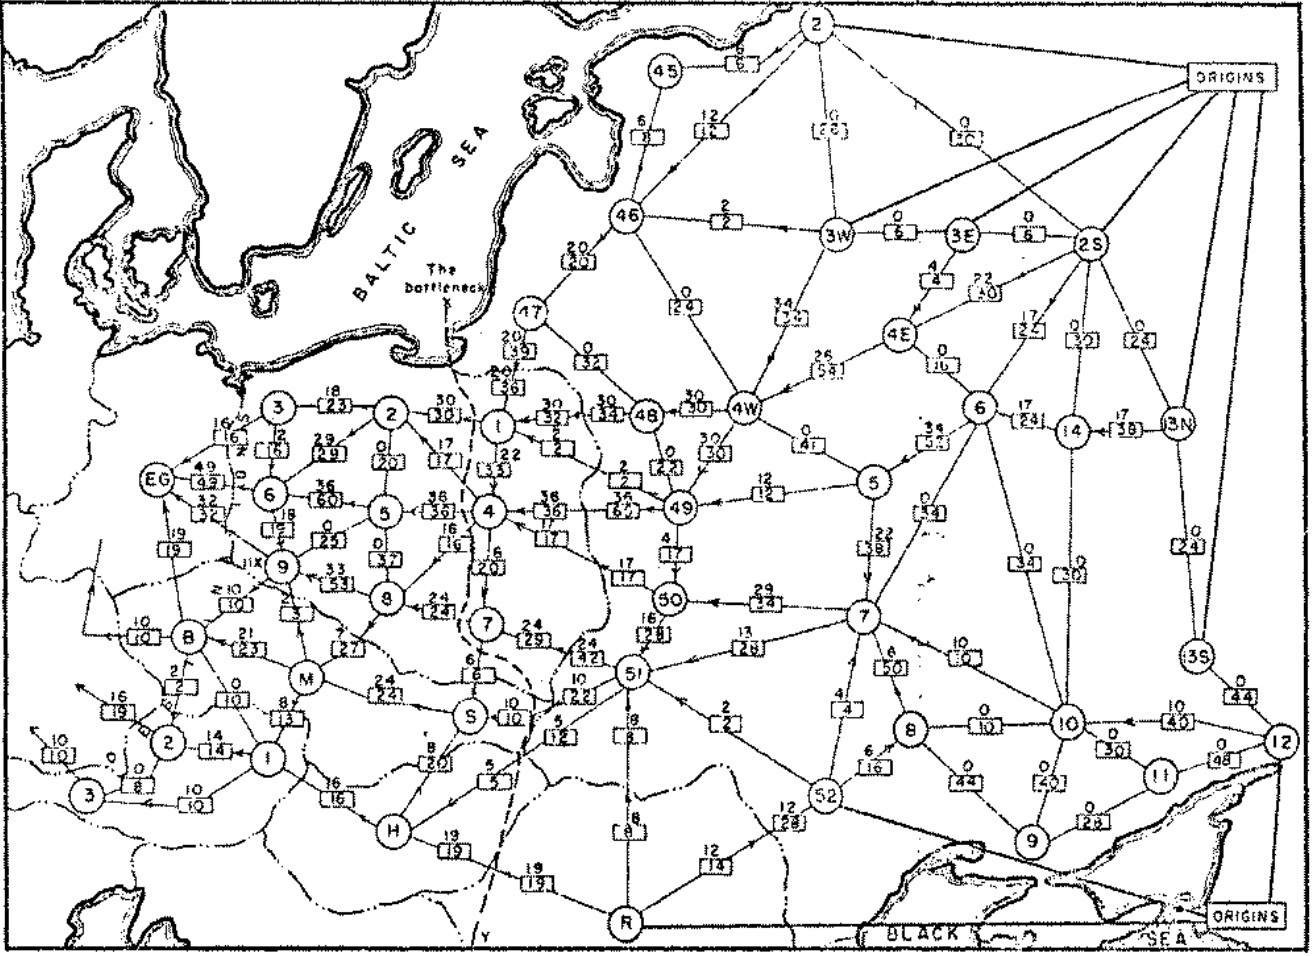
\includegraphics[scale=0.15]{soviettrainnetwork.jpeg}
\caption{\protect\bibentry{Schrijver02onthe}:\\
 Network flows and minimum cuts played a role in the Cold War. The figure is a schematic diagram of the railway network of the Western Soviet Union and Eastern European countries, with a maximum flow of value 163,000 tons from Russia to Eastern Europe, and a cut of capacity 163,000 tons indicated as “The bottleneck”.}
\end{figure}

\begin{defn}\label{networkcut}
In a network $(G, s, t, c)$ a \textbf{cut} is a partition of the vertex set $V$ into two subsets $S$ and $T$, such that $V = S \cup T$, $S \cap T = \emptyset$ and $s \in S, t \in T$. The \textbf{capacity} of the cut $(S, T)$, denoted $\|S,T\|$, is defined as

$$
\|S, T\| = \sum_{v \in S} \sum_{w \in T} c(v \rightarrow w)
$$
\end{defn}

\begin{thm}\label{flowcut}
With network $(G, s, t, c)$, for any flow $f$ and any cut $(S, T)$ we have
$$
  |f| \leq \|S, T\|
$$
Furthermore equality holds if and only if $f$ saturates every edge from $S$ to $T$ and avoids every edge from $T$ to $S$.
\end{thm}

\begin{proof}

\begin{align*}
|f| &= \sum_w f(s \rightarrow w) \tag*{\tiny{(by definition)}}\\
    &= \sum_w f(s \rightarrow w) - \sum_v f(v \rightarrow s) \tag*{\tiny{(second sum terms are all zero)}}\\
    &= \sum_{u \in S} (\sum_w f(u \rightarrow w) - \sum_v f(v \rightarrow u)) \tag*{\tiny{(flow conservation constraint)}}\\
    &= \sum_{u \in S} (\sum_{w \in T} f(u \rightarrow w) - \sum_{v \in T} f(v \rightarrow u)) \tag*{\tiny{(edges in $S$ cancel each other out)}}\\
    &\leq \sum_{u \in S} \sum_{w \in T} f(u \rightarrow w) \tag*{\tiny{(because $f(v \rightarrow u) \geq 0$)}}\\
    &\leq \sum_{u \in S} \sum_{w \in T} c(u \rightarrow w) \tag*{\tiny{(flow capacity constraint)}}\\
    &= \|S, T\| \tag*{\tiny{(by definition)}}
\end{align*}

\end{proof}

\begin{marginfigure}
\begin{tikzpicture}[
            shorten > = 1pt, % don't touch arrow head to node
            auto,
            semithick % line style
        ]

        \tikzstyle{every state}=[
            draw = black,
            thick,
            fill = white,
            minimum size = 4mm
        ]

        \node[state] (s) at (0,1) {$s$};
        \node[state] (v) at (2,2) {$v$};
        \node[state] (u) at (2,0) {$u$};
        \node[state] (t) at (4,1) {$t$};

        \path[->, line width=1.5pt] (s) edge node[below left=.05cm] {$20/20$} (u);
        \path[->] (s) edge node {$0/10$} (v);
        \path[->, line width=1.5pt] (u) edge node {$20/100$} (v);
		\path[->] (u) edge node[below right=.05cm] {$0/10$} (t);
		\path[->, line width=1.5pt] (v) edge node {$20/20$} (t);

		\path[->, dashed] (s) edge[bend left=60] node {$10$} (v);        
		\path[->, dashed] (v) edge[bend left=30] node {$20$} (u);
		\path[->, dashed] (u) edge[bend right=70] node[right] {$10$} (t);  

    \end{tikzpicture}
    \caption{Dashed edges show how the greedy $s-t$ path flow can be augmented and reversed in order to increase overall flow.}
	\label{ex_flow_dashed}
\end{marginfigure}

Theorem \ref{flowcut} tells us that if we keep increasing a flow and/or decreasing a cut we should eventually meet at a maximum flow that equals a minimum cut. But given a network how do we start? A first valid flow is $\forall e \in E: f(e) = 0$. We could then try a greedy strategy. Starting with source $s$ find the path to $t$ with the biggest capacity\footnote{The capacity of a path is the minimum over the capacities of the edges forming the path.} and pump as much flow as we can through it as illustrated in Figure \ref{ex_flow}. Unfortunately we are stuck at that point. We cannot pump more flow out of $s$ on $s \rightarrow v$ because that would violate flow conservation at $v$ (we are at the maximum outgoing flow at $v$). The dashed edges in Figure \ref{ex_flow_dashed} show some of our options. On edges where the current flow leaves residual capacity we can pump more and on edges where there is existing flow we can reverse it. Again, this concept seems worth formalizing.

\begin{defn}\label{residualgraph}
A flow $f$ in a network $(G, s, t, c)$ induces a \textbf{residual network} $(G_f, s, t, c_f)$ with \textbf{residual graph} $G_f$ and \textbf{residual capacity} $c_f$ in the following way:

\begin{itemize}
	\item all vertices from $G$ are vertices in $G_f$, also source $s$ and target $t$ are the same in $G$ and $G_f$
	\item if $f(u \rightarrow v) > 0$ then $G_f$ has an edge $(v \rightarrow u)$ with capacity 
$$
c_f(v \rightarrow u) = f(u \rightarrow v)
$$
    \item if $f(u \rightarrow v) < c(u \rightarrow v)$ then $G_f$ has an edge $(u \rightarrow v)$ with capacity
$$
c_f(u \rightarrow v) = c(u \rightarrow v) - f(u \rightarrow v)
$$
\end{itemize}

\end{defn}

Figure \ref{ex_residual} shows the residual network of our example network and flow. We observe that there is a simple path\footnote{A simple path is a path where every vertex on the path is visited only once.} $s \rightarrow v \rightarrow u \rightarrow t$ with capacity $10$ from source $s$ to target $t$ in the residual graph. This path shows that there still is unused capacity for flow to be pushed from $s$ to $t$. A simple path from $s$ to $t$ in $G_f$ is called an \textbf{augmenting path}.

\begin{marginfigure}
\begin{tikzpicture}[
            shorten > = 1pt, % don't touch arrow head to node
            auto,
            semithick % line style
        ]

        \tikzstyle{every state}=[
            draw = black,
            thick,
            fill = white,
            minimum size = 4mm
        ]

        \node at (0,2.7) {(a)};
        \node at (0,0) {(b)};

        \node[state] (sf) at (0,1) {$s$};
        \node[state] (vf) at (2,2) {$v$};
        \node[state] (uf) at (2,0) {$u$};
        \node[state] (tf) at (4,1) {$t$};

        \node[state] (s) at (0,4) {$s$};
        \node[state] (v) at (2,5) {$v$};
        \node[state] (u) at (2,3) {$u$};
        \node[state] (t) at (4,4) {$t$};

        \path[->] (s) edge node[below left=.05cm] {$20/20$} (u);
        \path[->] (s) edge node {$0/10$} (v);
        \path[->] (u) edge node {$20/100$} (v);
		\path[->] (u) edge node[below right=.05cm] {$0/10$} (t);
		\path[->] (v) edge node {$20/20$} (t);

        \path[<-, blue] (sf) edge node[below left=.05cm] {$20$} (uf);
        \path[->, blue] (sf) edge node {$10$} (vf);
        \path[->, blue] (uf) edge[bend left=30] node {$80$} (vf);
        \path[<-, blue] (uf) edge[bend right=30] node {$20$} (vf);
		\path[->, blue] (uf) edge node[below right=.05cm] {$10$} (tf);
		\path[<-, blue] (vf) edge node {$20$} (tf);

    \end{tikzpicture}
    \caption{\\
             (a) Example network with flow from Figure \ref{ex_flow}. \\
             (b) Residual network (in blue) with edges annotated with their residual capacity.}
	\label{ex_residual}
\end{marginfigure}


\begin{marginfigure}
\begin{tikzpicture}[
            shorten > = 1pt, % don't touch arrow head to node
            auto,
            semithick % line style
        ]

        \tikzstyle{every state}=[
            draw = black,
            thick,
            fill = white,
            minimum size = 4mm
        ]

        \node at (0,2.7) {(a)};
        \node at (0,0) {(b)};

        \node[state] (sf) at (0,1) {$s$};
        \node[state] (vf) at (2,2) {$v$};
        \node[state] (uf) at (2,0) {$u$};
        \node[state] (tf) at (4,1) {$t$};

        \node[state] (s) at (0,4) {$s$};
        \node[state] (v) at (2,5) {$v$};
        \node[state] (u) at (2,3) {$u$};
        \node[state] (t) at (4,4) {$t$};

        \path[->] (s) edge node[below left=.05cm] {$20/20$} (u);
        \path[->] (s) edge node {$0/10$} (v);
        \path[->] (u) edge node {$20/100$} (v);
		\path[->] (u) edge node[below right=.05cm] {$0/10$} (t);
		\path[->] (v) edge node {$20/20$} (t);

		\path[->] (sf) edge node[below left=.05cm] {$20/20$} (uf);
        \path[->] (sf) edge node {$\color{red}10\color{black}/10$} (vf);
        \path[->] (uf) edge node {$\color{red}10\color{black}/100$} (vf);
		\path[->] (uf) edge node[below right=.05cm] {$\color{red}10\color{black}/10$} (tf);
		\path[->] (vf) edge node {$20/20$} (tf);

    \end{tikzpicture}
    \caption{\\
             (a) Example network with flow from Figure \ref{ex_flow}. \\
             (b) Augmented flow (changed values in red) from augmenting path $s \rightarrow v \rightarrow u \rightarrow t$.}
	\label{augmented_flow}
\end{marginfigure}

\begin{thm}\label{augmenting}
Given is a flow $f$ in network $(G, s, t, c)$. If there is an augmenting path in $G_f$ with capacity $F$ then the function $f':V \times V \to \mathbb{R}_{\geq 0}$ defined as:

$$
f'(u \rightarrow v) = 
\begin{cases}
f(u \rightarrow v) + F, & \text{if } u\rightarrow v \text{ is on the augmenting path} \\
f(u \rightarrow v) - F, & \text{if } v\rightarrow u \text{ is on the augmenting path} \\
f(u \rightarrow v), & \text{otherwise}
\end{cases}
$$

is a valid flow in network $(G, s, t, c)$ with $|f'| = |f| + F$.
\end{thm}

\begin{proof}
We need to check the capacity constraint and the conservation constraint. 

Let's start with the capacity constraint. The definition of $f'$ has three cases, so we check all three:

\begin{itemize}

	\item Edge $u \rightarrow v$ is on the augmenting path:

\begin{align*}
f'(u \rightarrow v) &= f(u \rightarrow v) + F \tag*{\tiny{(by definition)}}\\
    &\leq f(u \rightarrow v) + c_f(u \rightarrow v) \tag*{\tiny{(by definition of $F$)}}\\
    &=  f(u \rightarrow v) + c(u \rightarrow v) - f(u \rightarrow v) \tag*{\tiny{(by definition of $c_f$)}}\\
    &=  c(u \rightarrow v)
\end{align*}

	\item Edge $v \rightarrow u$ is on the augmenting path:

\begin{align*}
f'(u \rightarrow v) &= f(u \rightarrow v) - F \tag*{\tiny{(by definition)}}\\
    &\geq f(u \rightarrow v) - c_f(u \rightarrow v) \tag*{\tiny{(by definition of $F$)}}\\
    &=  f(u \rightarrow v) - f(u \rightarrow v) \tag*{\tiny{(by definition of $c_f$)}}\\
    &=  0
\end{align*}

	\item Otherwise: In this case the flow of the edge hasn't changed so capacity constraint is satisfied.

\end{itemize}

Next is the conservation constraint. For vertices not on the augmenting path flow in and out of them hasn't changed, so conservation constraint is satisfied there. For a vertex $v$ on the augmenting path we have four cases (since the augmenting path is simple and $v \neq s, v \neq t$):

\begin{itemize} 

	\item $u \rightarrow v$ on augmenting path and $v \rightarrow w$ on augmenting path: in this case one incoming edge into $v$ changed by $F$ and one outgoing changed by $F$, so conservation constraint holds for $v$

	\item $u \rightarrow v$ on augmenting path and $w \rightarrow v$ on augmenting path: in this case two incoming edges into $v$ changed, one by $F$ and the other by $-F$, so conservation constraint holds for $v$

	\item $v \rightarrow u$ on augmenting path and $w \rightarrow v$ on augmenting path: in this case one incoming edge into $v$ changed by $-F$ and one outgoing changed by $-F$, so conservation constraint holds for $v$

	\item $v \rightarrow u$ on augmenting path and $v \rightarrow w$ on augmenting path: in this case two outgoing edges from $v$ changed, one by $-F$ and the other by $F$, so conservation constraint holds for $v$

\end{itemize}	

\end{proof}

\begin{marginfigure}
\begin{tikzpicture}[
            shorten > = 1pt, % don't touch arrow head to node
            auto,
            semithick % line style
        ]

        \tikzstyle{every state}=[
            draw = black,
            thick,
            fill = white,
            minimum size = 4mm
        ]

        \node at (0,2.7) {(a)};
        \node at (0,0) {(b)};

        \node[state] (sf) at (0,1) {$s$};
        \node[state] (vf) at (2,2) {$v$};
        \node[state] (uf) at (2,0) {$u$};
        \node[state] (tf) at (4,1) {$t$};

        \node[state] (s) at (0,4) {$s$};
        \node[state] (v) at (2,5) {$v$};
        \node[state] (u) at (2,3) {$u$};
        \node[state] (t) at (4,4) {$t$};

        \path[->] (s) edge node[below left=.05cm] {$20/20$} (u);
        \path[->] (s) edge node {$10/10$} (v);
        \path[->] (u) edge node {$10/100$} (v);
		\path[->] (u) edge node[below right=.05cm] {$10/10$} (t);
		\path[->] (v) edge node {$20/20$} (t);

        \path[<-, blue] (sf) edge node[below left=.05cm] {$20$} (uf);
        \path[<-, blue] (sf) edge node {$10$} (vf);
        \path[->, blue] (uf) edge[bend left=30] node {$90$} (vf);
        \path[<-, blue] (uf) edge[bend right=30] node {$10$} (vf);
		\path[<-, blue] (uf) edge node[below right=.05cm] {$10$} (tf);
		\path[<-, blue] (vf) edge node {$20$} (tf);

    \end{tikzpicture}
    \caption{\\
             (a) Example network with flow from Figure \ref{ex_flow_max}. \\
             (b) Residual network (in blue) with edges annotated with their residual capacity.}
	\label{ex_residual_max}
\end{marginfigure}

What happens when there is no augmenting path in $G_f$? As the Figure \ref{ex_residual_max} hints we then have a maximum flow (in our example $|f| = 30$). The next theorem proves it.

\begin{thm}\label{no_augmenting}
Given is a flow $f$ in network $(G, s, t, c)$. If there is no augmenting path in $G_f$ then $f$ is a flow with maximum value.
\end{thm}

\begin{proof}
We define two subsets of $V$. The set $S$ holds all the vertices of $V$ that are reachable from $s$ in $G_f$. Since there is no augmenting path in $G_f$ we have $t \notin S$. We also define $T = V \setminus S$. Clearly $(S, T)$ is a cut of our network. Also there is no $G_f$ edge $u \rightarrow v$ with $u \in S$ and $v \in T$ because otherwise $v$ would be reachable from somewhere in $S$ but $v \notin S$, contradicting the definition of $S$. This means (by definition of $G_f$) that $f$ saturates every edge from $S$ to $T$ and avoids every edge from $T$ to $S$. According to Theorem \ref{flowcut} we then have $|f| = \|S, T\|$ which means we have a maximum flow and minimum cut.

\end{proof}

\begin{marginfigure}
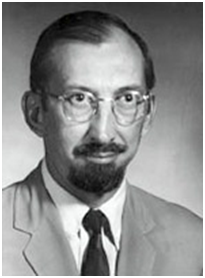
\includegraphics[scale=0.8]{fulkerson.png}
\end{marginfigure}
\marginnote{Delbert Ray Fulkerson was an American mathematician who co-developed the Ford–Fulkerson algorithm. \url{https://en.wikipedia.org/wiki/D._R._Fulkerson}}

We can now piece together the following algorithm known as the \textbf{Ford-Fulkerson algorithm}:

\begin{lstlisting}[basicstyle=\small, label={lst:fordfulkerson}, frame=trBL, caption={Ford-Fulkerson algorithm}]
f = zero flow;
Gf = residual graph of f in G;

while (exists augmenting path in Gf):
   pa = choose any augmenting path; 
   f = augment f with pa;
   Gf = residual graph of f in G;

return f  
\end{lstlisting}

\begin{thm}\label{fordfulkerson}
If the network has capacities in $\mathbb{N}_{\geq 0}$ then the Ford-Fulkerson algorithm terminates and returns the maximum flow in the network.
\end{thm}

\begin{proof}
We prove by induction that $f: V \times V \to \mathbb{N}_{\geq 0}$: The base case is the zero flow which is in $\mathbb{N}_{\geq 0}$. Assume the current flow values are in $\mathbb{N}_{\geq 0}$. The augmenting operation adds or subtracts a positive integer value from the current flow values and conforms to capacity constraints, so it keeps the augmented flow values in $\mathbb{N}_{\geq 0}$ which completes the induction.

The augmented flow $f'$ modifies one outgoing edge from $s$ by $F > 0$, so by the definition of the value of a flow we have $|f'| = |f| + F$. This means that augmenting strictly increases the value of the flow. We also know that flow values have an upper bound (by Theorem \ref{flowcut} any cut capacity is an upper bound). This means the algorithm has to eventually reach the maximum flow and terminate.
\end{proof}

\newpage

This concludes our detour into network flows\footnote{We have just scratched the surface of the topic on network flows and algorithms computing maximum flows (an area of active research). For example by making smart choices when choosing the augmenting path we can improve the runtime of the algorithm (also we haven't analyzed the runtime). What happens when the capacities are not in $\mathbb{N}_{\geq 0}$. For details on all this and more see:
\\
\bibentry{kleinberg2005ad} 
\\ 
\bibentry{erickson2015a}.}.
\\
We should bring it back to our problem and the associated bipartite graph of conflicting votes. We want a minimal vertex cover and we would like to use the just derived Ford-Fulkerson algorithm to compute it. So we first have to transform our undirected bipartite graph into a network. 

We have an undirected bipartite graph $G(V = X \cup Y, E)$ with $X \cap Y = \emptyset$ and $E \subseteq X \times Y$ ($X$ could be the votes of cat lovers and $Y$ the votes of dog lovers in our problem or vice versa). We add a source $s$ and a target $t$ and construct a network $(G', s, t, c)$ in the following way:

\begin{itemize}
	\item vertex set of $G'$ is $X \cup Y \cup \{s, t\}$
	\item $\forall u \in X$ add a directed edge $s \rightarrow u$ into edge set of $G'$
	\item $\forall v \in Y$ add a directed edge $v \rightarrow t$ into edge set of $G'$
	\item $\forall \{u, v\}$ undirected edge in $G$ with $u \in X$ and $v \in Y$ add a directed edge $u \rightarrow v$  into edge set of $G'$
	\item unit capacity\footnote{Unit capacity has the advantage that a flow either saturates the edge or avoids it.}: $\forall (u \rightarrow v) \in \text{ edge set of } G': c(u \rightarrow v) = 1$
\end{itemize}

With a network $(G', s, t, c)$ constructed from a bipartite graph $G$ as described above (an example is shown in Figure \ref{bipartite_network}) we have an equivalence between a matching in the bipartite graph and a flow in the network. The next theorem states this.

\begin{marginfigure}
\begin{tikzpicture}[
            shorten > = 1pt, % don't touch arrow head to node
            auto,
            semithick % line style
        ]

        \tikzstyle{every state}=[
            draw = black,
            thick,
            fill = white,
            minimum size = 4mm
        ]

        \node at (0,4.5) {(a)};
        \node at (0,0) {(b)};

        \node[state] (s) at (0,3) {$s$};
        \node[state] (t) at (5,3) {$t$};

        \node[state] (x1) at (1.5,0.5) {$x_1$};
        \node[state] (x2) at (1.5,2) {$x_2$};
        \node[state] (x3) at (1.5,3) {$x_3$};
        \node[state] (x4) at (1.5,4) {$x_4$};

        \node[state] (y1) at (3,0.5) {$y_1$};
        \node[state] (y2) at (3,2) {$y_2$};
        \node[state] (y3) at (3,3) {$y_3$};

        \path[->] (x1) edge node {$1$} (y1);
        \path[->] (x2) edge node {$1$} (y1);
        \path[->] (x2) edge node {$1$} (y2);
        \path[->] (x2) edge node {$1$} (y3);
        \path[->] (x3) edge node {$1$} (y3);
        \path[->] (x4) edge node {$1$} (y3);

        \path[->] (s) edge node {$1$} (x1);
        \path[->] (s) edge node {$1$} (x2);
        \path[->] (s) edge node {$1$} (x3);
        \path[->] (s) edge node {$1$} (x4);

        \path[->] (y1) edge node {$1$} (t);
        \path[->] (y2) edge node {$1$} (t);
        \path[->] (y3) edge node {$1$} (t);

        \node[state] (bx1) at (1.5,5.5) {$x_1$};
        \node[state] (bx2) at (1.5,7) {$x_2$};
        \node[state] (bx3) at (1.5,8) {$x_3$};
        \node[state] (bx4) at (1.5,9) {$x_4$};

        \node[state] (by1) at (3,5.5) {$y_1$};
        \node[state] (by2) at (3,7) {$y_2$};
        \node[state] (by3) at (3,8) {$y_3$};

        \path[-] (bx1) edge node {} (by1);
        \path[-] (bx2) edge node {} (by1);
        \path[-] (bx2) edge node {} (by2);
        \path[-] (bx2) edge node {} (by3);
        \path[-] (bx3) edge node {} (by3);
        \path[-] (bx4) edge node {} (by3);

    \end{tikzpicture}
    \caption{\\
             (a) Bipartite graph \\
             (b) Network constructed from it.}
	\label{bipartite_network}
\end{marginfigure}

\begin{thm}\label{matchingflow}
A matching $M$ in $G$ induces a flow $f$ in $G'$ such that $|f| = |M|$. Conversely a flow in $G'$ induces a matching $M$ in $G$ such that $|M| = |f|$.
\end{thm}

\begin{proof}
\noindent$(\Rightarrow)$ We have a matching $M$ in $G$, i.e. a subset of edges that don't share a vertex. From the construction of $G'$ it follows that each of the edges in $M$ can be extended to paths from $s$ to $t$ which will only meet in $s$ and $t$. We define a function $f$ that gives unit values to the edges along these paths and zero value to all other edges. We claim that $f$ is a valid flow. It only assigns zero or unit values so it does satisfy the capacity constraint in $G'$. The paths don't intersect except in $s$ and $t$ (because $M$ is a matching), so for any vertex along the path there is exactly one incoming edge with unit value and one outgoing edge with unit value. The rest of the edges have value zero so don't play a role in conservation. This then means that the conservation constraint is satisfied also and $f$ is a flow.
Each edge in $M$ corresponds to one of the paths, so there are $|M|$ edges outgoing from $s$ that have unit value. Hence $|f| = |M|$.

\noindent$(\Leftarrow)$ We have a flow $f$ in $G'$. The flow either saturates or avoids an edge. We define the subset $M$ of edges that are saturated by $f$ and are between $X$ and $Y$. We claim that $M$ is a matching in $G$. Suppose it is not a matching. Then there exists a vertex that is shared by two edges in $M$. If this vertex is in $X$ then it means it has two outgoing edges of unit value but only one incoming edge of unit value (from $s$). If this vertex is in $Y$ then it means it has two incoming edges of unit value and only one outgoing edge of unit value (to $t$). In either case this is a contradiction to the conservation constraint of $f$. So $M$ has to be a matching. The size of $M$ is by its definition equal to the number of saturated edges from $X$ to $Y$. But this number has to be equal to the number of edges of unit value going out of $s$ (conservation constraint). Hence $|M| = |f|$.
\end{proof}

Theorem \ref{matchingflow} let's us use the Ford-Fulkerson algorithm to compute a maximum matching in our bipartite graph $G$. Once we have a maximum matching we get the size of a minimum vertex cover with the following theorem, known as \textbf{K\"onig's theorem}\footnote{For a short and elegant proof see:\\\bibentry{rizzi00}}:

\begin{thm}\label{koenig}
In a bipartite graph $G$ the size of a minimum vertex cover $C$ equals the size of a maximum matching $M$. 
\end{thm}

\begin{proof}

$C$ is a vertex cover, so it covers all edges, which means it certainly covers a subset $M$ of all edges. But $M$ is a matching, so no two edges share a vertex. It follows that $|C| \geq |M|$.

From the maximum matching $M$ we get the associated maximum flow $f$ as described in Theorem \ref{matchingflow}. The residual graph $G'_f$ of the associated network cannot have any augmenting paths. 

We consider the minimum cut $(S, T)$ associated with the maximum flow $f$. We define the following sets:

\begin{itemize}
	\item $X_S = X \cap S, X_T = X \cap T$
	\item $Y_S = Y \cap S, Y_T = Y \cap T$
	\item $H = \{(u, v) \text{ edge in } G: u \in S, v \in T\}$
	\item $B = \{v \in Y_T: \exists u \in X_S \text{ with } (u, v) \text{ edge in } G\}$
	\item $D = X_T \cup Y_S \cup B$
\end{itemize}	

\noindent $D$ is a vertex cover: $X_T \subseteq D$ and $Y_S \subseteq D$, so $D$ covers all edges that have endpoints in $X_T$ or $Y_S$. The set $B$ provides cover for $H$. 

A vertex $u \in X_T$ is not reachable from $s$ in $G'_f$. It means that $f$ saturates $s \rightarrow u$ in $G'$, so the saturated edge $s \rightarrow u$ crosses the $(S, T)$ cut and counts towards $\|S, T\|$.

A vertex $v \in Y_S$ is reachable from $s$ in $G'_f$. It means that $f$ saturates $v \rightarrow t$ in $G'$ (otherwise some vertex from $T$ would be reachable from $v$ and also from $s$ in $G'_f$ which is a contradiction). The saturated edge $v \rightarrow t$ crosses the $(S, T)$ cut and counts towards $\|S, T\|$.

$f$ is a maximum flow so any edge from $X_S$ to $Y_T$ is saturated and counts towards $\|S, T\|$.

\begin{figure}[t]
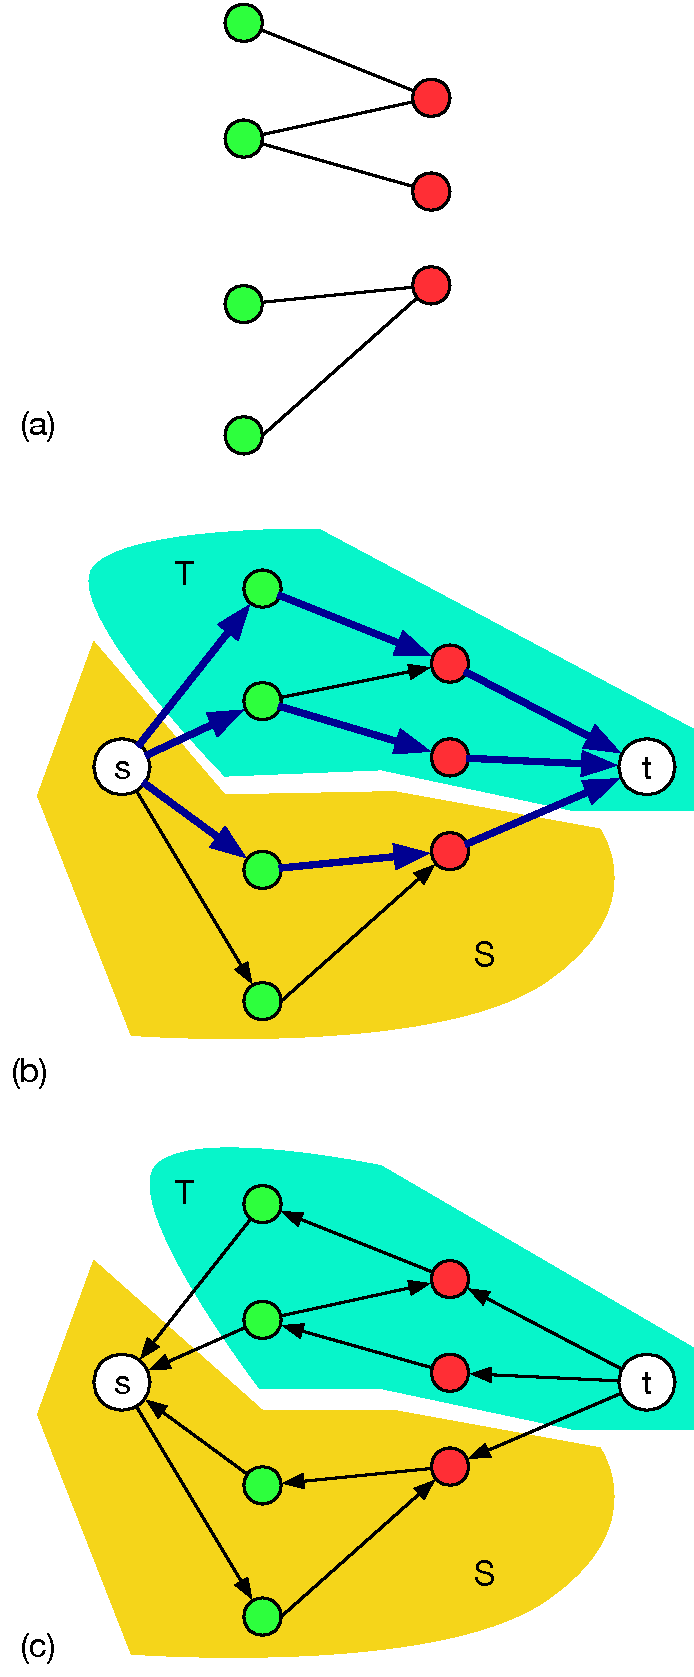
\includegraphics[scale=0.5]{koenig.pdf}
\caption{\\
             (a) A bipartite graph $G(X \cup Y, E)$. $X$ are green vertices, $Y$ are red vertices.\\
             (b) Maximum flow $f$ (thicker arrows) and minimum cut $(S, T)$ in the corresponding network $G'$. Thicker arrows between green and red vertices form the maximum matching.\\
             (c) Same cut displayed with the corresponding residual graph $G'_f$.}
	\label{koenig_example}
\end{figure}

$$
\|S, T\| = |X_T| + |Y_S| + |H|
$$

\noindent Figure \ref{koenig_example} shows this. In (b) there are three saturated (thick) arrows crossing the cut. The first two (counting from left to right) are due to $X_T$ and the last one due to $Y_S$. In this example $H$ is the empty set.

We have
$$
|M| = |f| = \|S, T\| = |X_T| + |Y_S| + |H| \geq |X_T| + |Y_S| + |B| \geq |D|
$$
\noindent $D$ is a vertex cover and $C$ is a minimum vertex cover, so $|D| \geq |C|$. It follows that $|C| \geq |M| \geq |D| \geq |C|$ which means $|C| = |M|$.
\end{proof}

This solves the problem in this note. The number of satisfied viewers is $|V| - |M|$, where $V$ is the set of vertices in the bipartite graph $G$ of votes with their conflicts as edges and $M$ is a maximum matching in $G$ computed with the Ford-Fulkerson algorithm taking advantage of the min-max duality shown in Figure \ref{minmax_duality}.

\begin{marginfigure}
    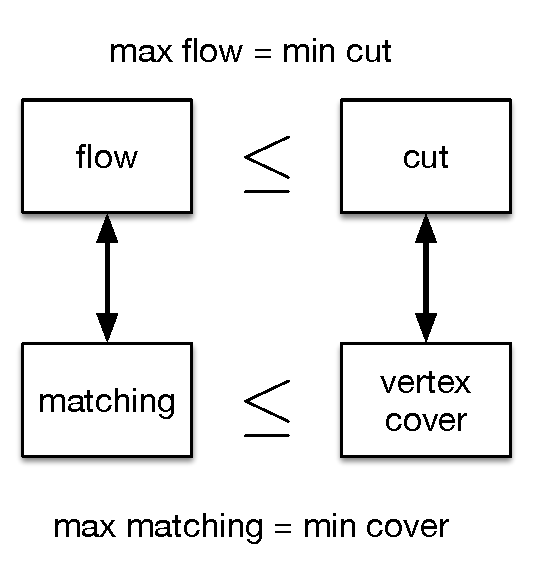
\includegraphics[scale=0.5]{flowcutminmax.pdf}
    \caption{Min-max duality in bipartite graphs and corresponding networks.}
	\label{minmax_duality}
\end{marginfigure}{}
